% Bagian Lampiran
\section*{Lampiran} % Jika ada lampiran

\begin{figure}[H]
  \centering
  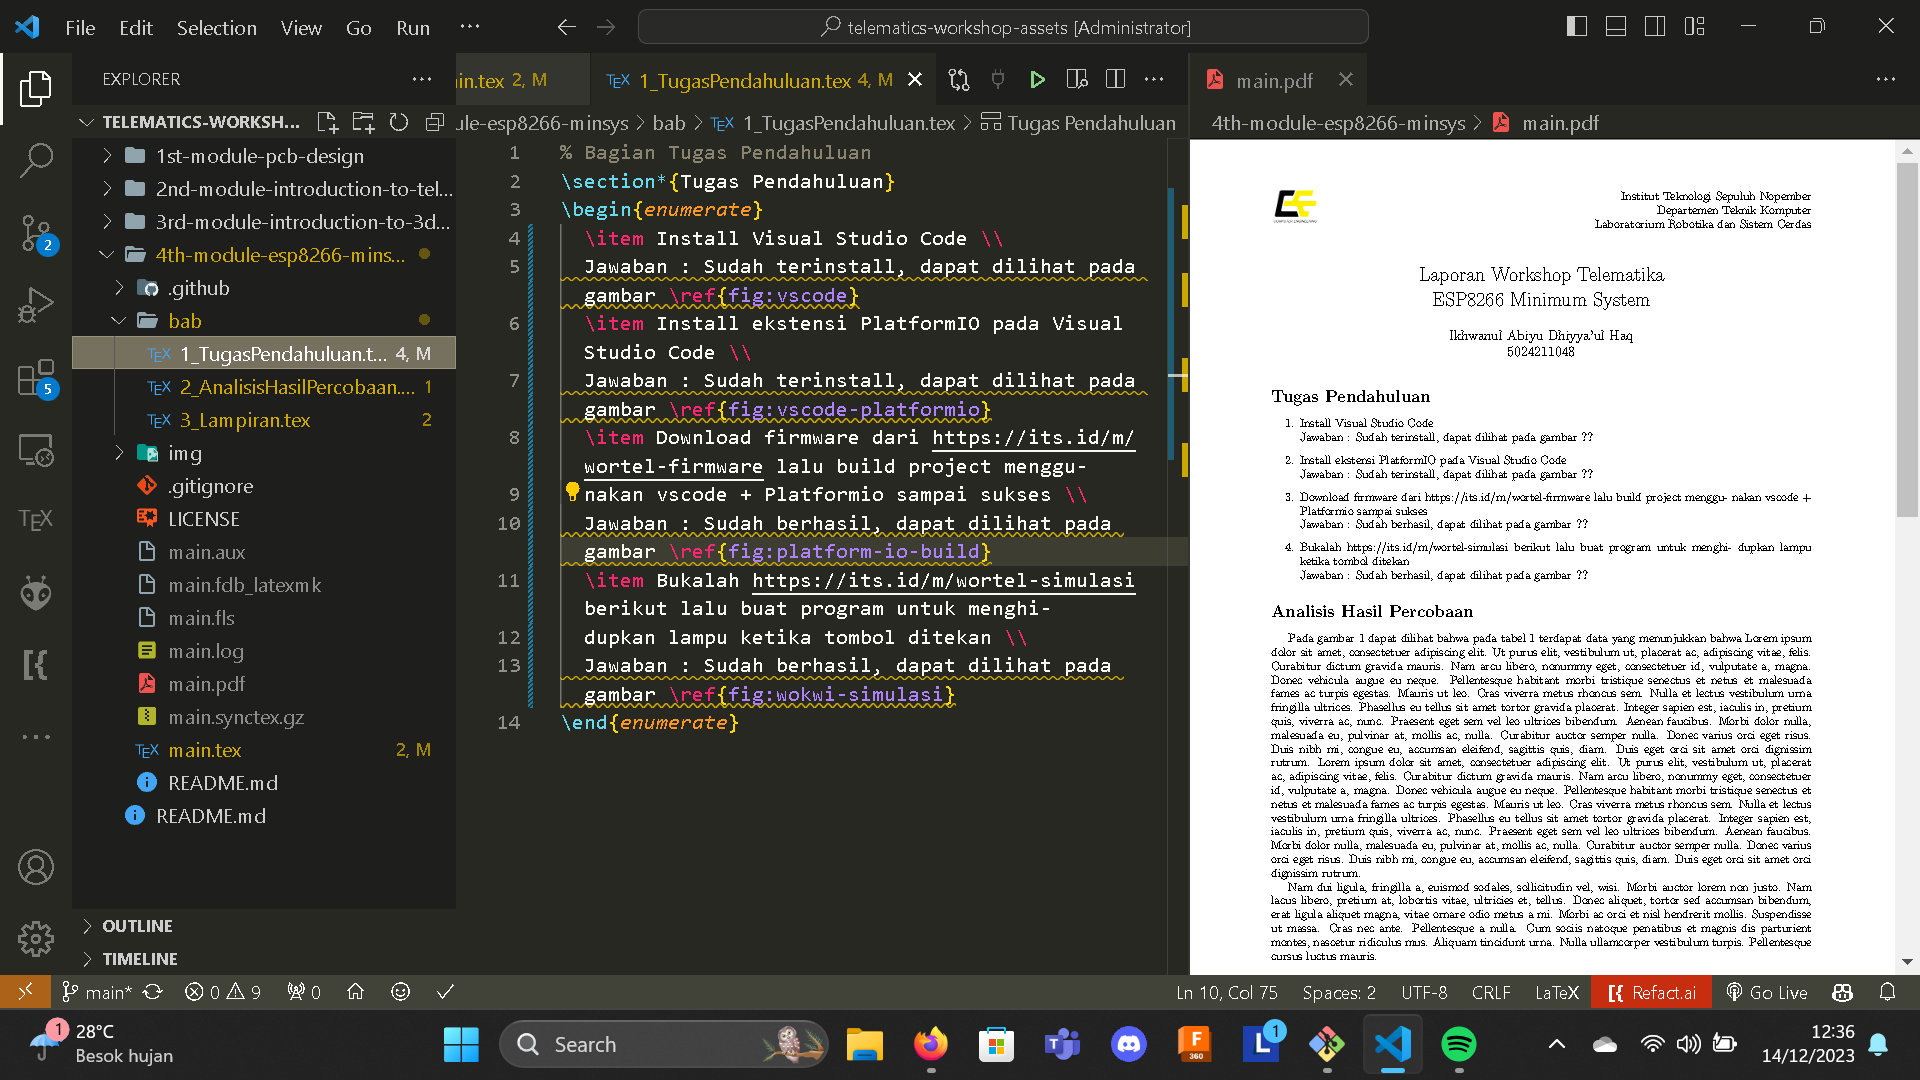
\includegraphics[width=0.8\textwidth]{img/vscode-install.png}
  \caption{Visual Studio Code yang sudah terinstall}
  \label{fig:vscode}
\end{figure}

\begin{figure}[H]
  \centering
  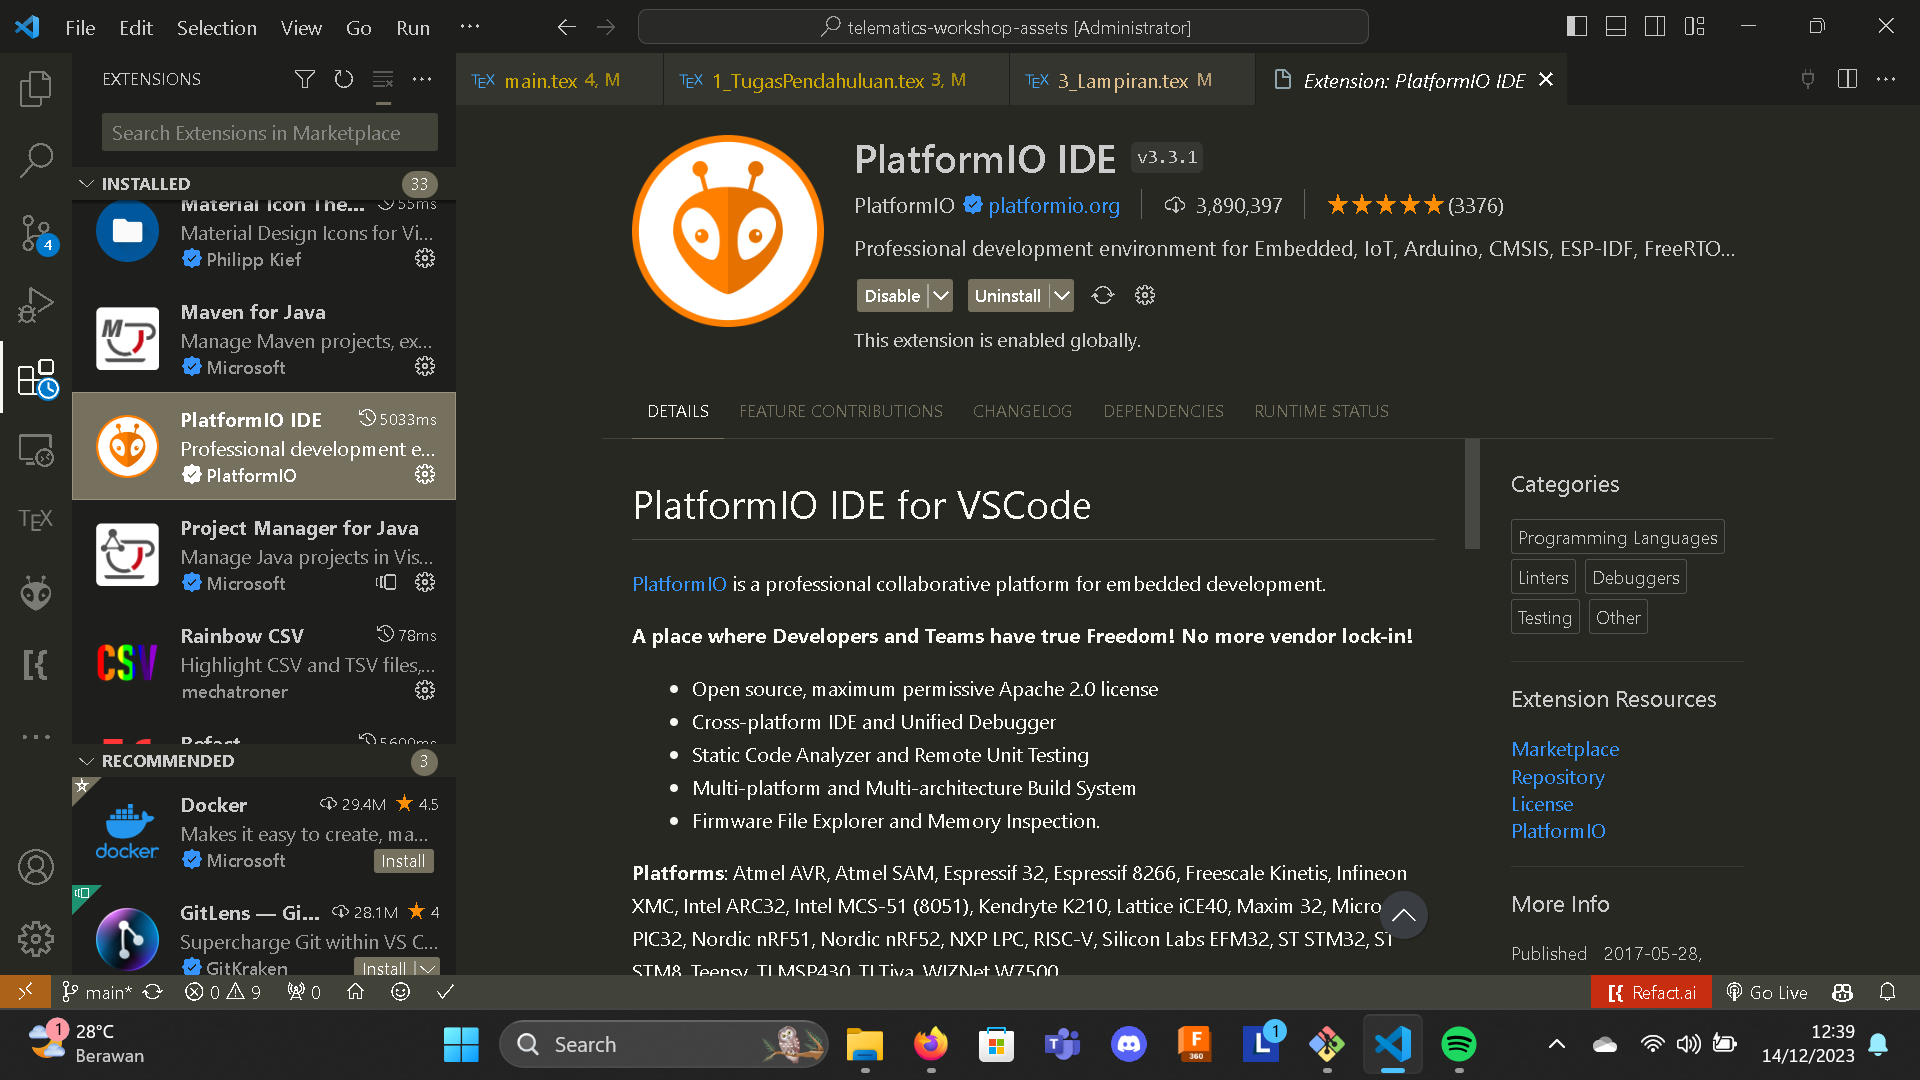
\includegraphics[width=0.8\textwidth]{img/platformio.png}
  \caption{Ekstensi PlatformIO pada Visual Studio Code yang sudah terinstall}
  \label{fig:vscode-platformio}
\end{figure}

\begin{figure}[H]
  \centering
  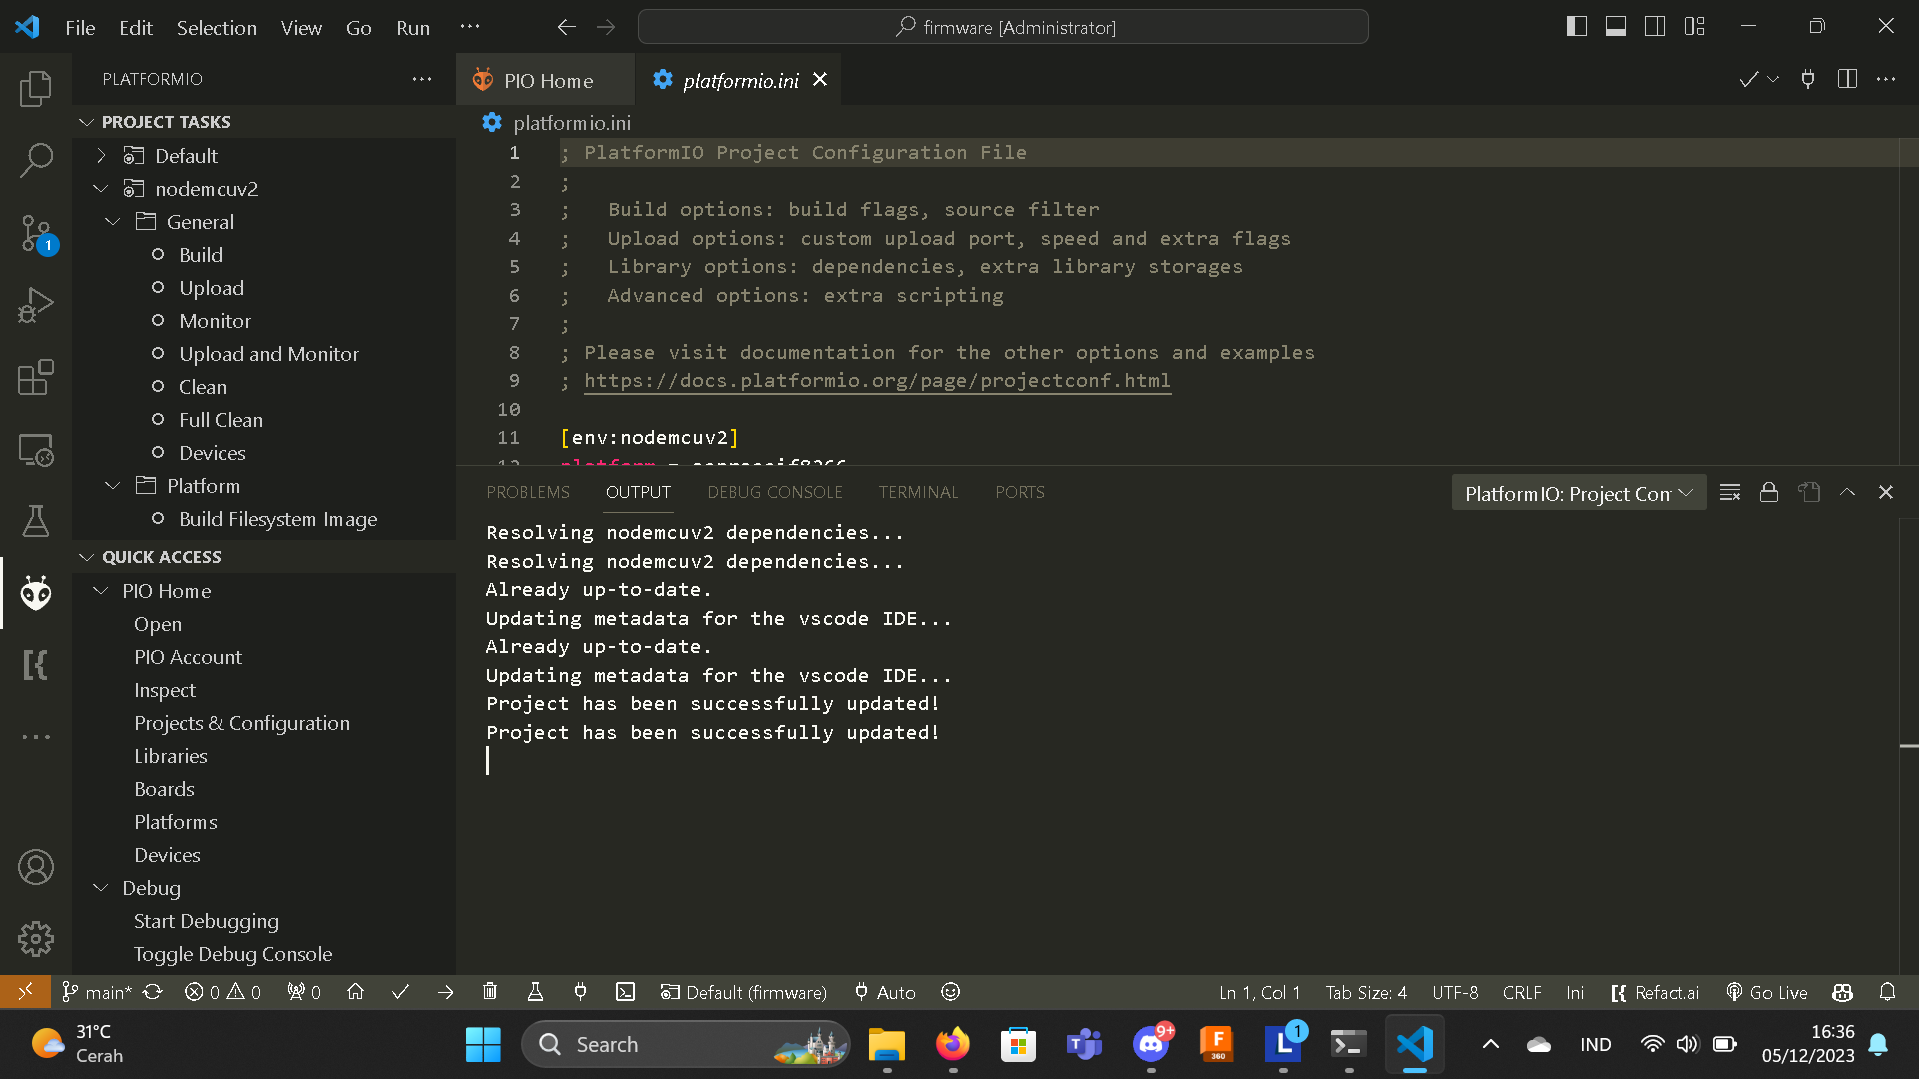
\includegraphics[width=0.8\textwidth]{img/platformio-build.png}
  \caption{PlatformIO berhasil melakukan build}
  \label{fig:platform-io-build}
\end{figure}

\begin{figure}[H]
  \centering
  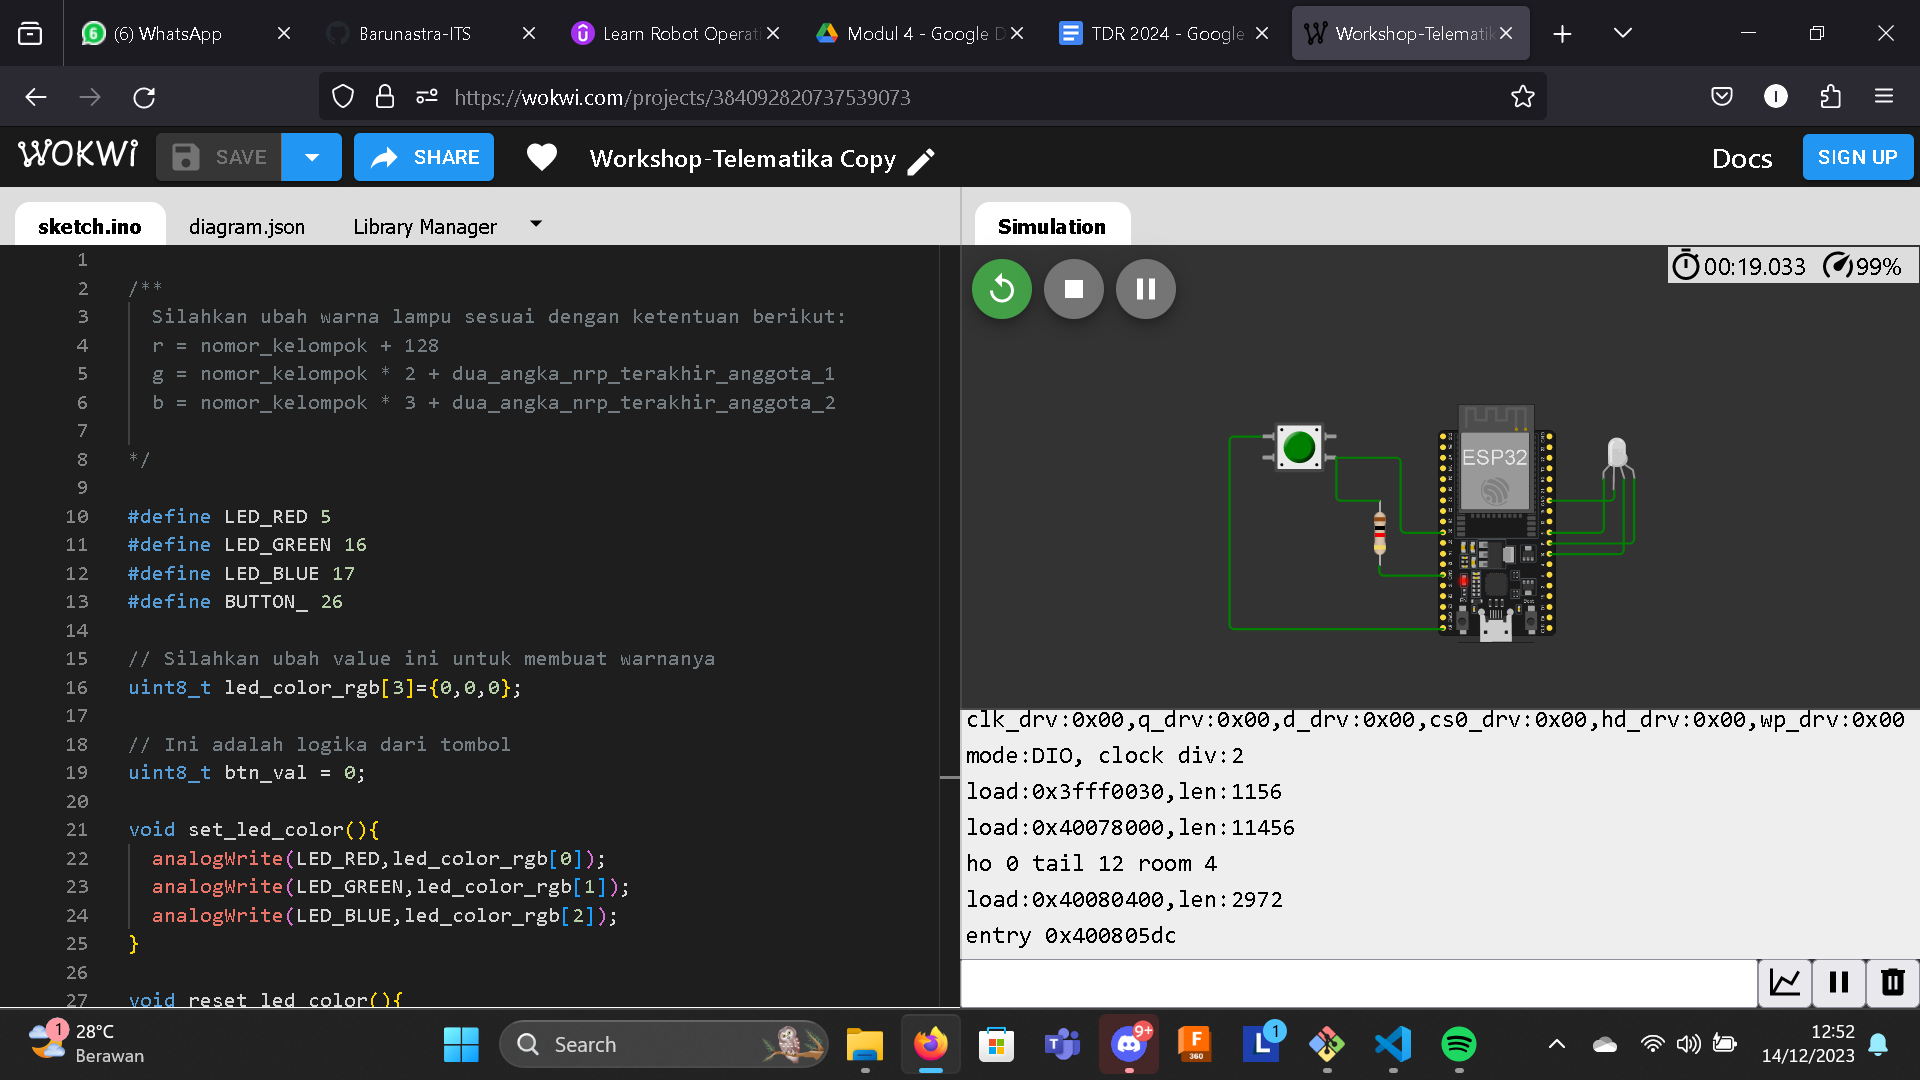
\includegraphics[width=0.8\textwidth]{img/wokwi-simulation.png}
  \caption{Wokwi berhasil melakukan simulasi}
  \label{fig:wokwi-simulasi}
\end{figure}

\begin{figure}[H]
  \centering
  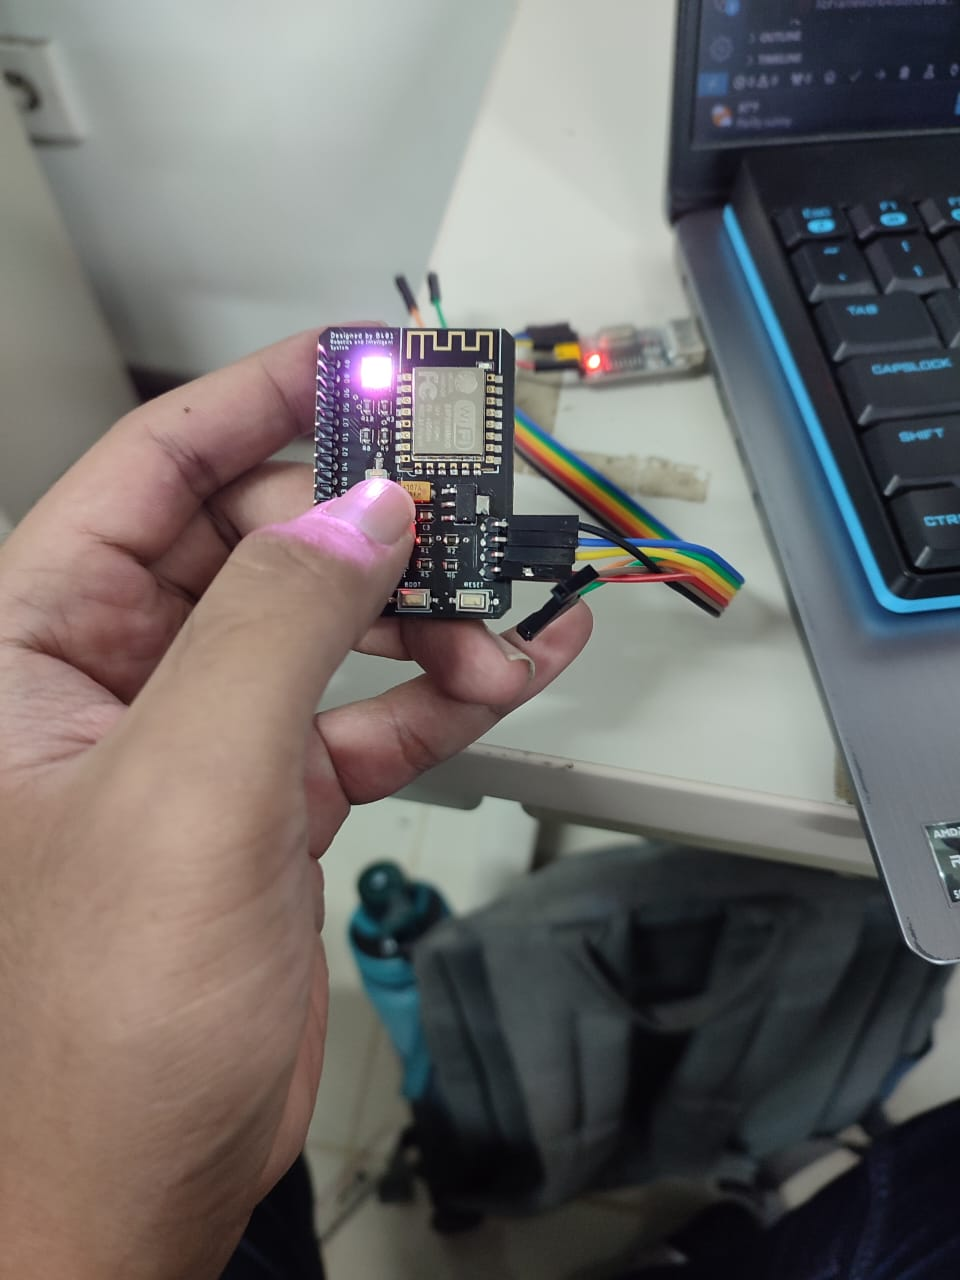
\includegraphics[width=0.8\textwidth]{img/esp-jadi.jpeg}
  \caption{ESP dengan program yang sudah diupload}
  \label{fig:ESP-jadi}
\end{figure}